\chapter{Experiment and Result}
brief of experiment and result.
\section{Experiment}
Please tell how the experiment conducted from method.

\section{Result}
Please provide the result of experiment

\section{Aip Suprapto Munari/1164063}

\subsection{Teori}
\begin{enumerate}
\item Klasifikasi teks
	\par Klasifikasi teks atau kategorisasi teks merupakan proses yang secara otomatis menempatkan dokumen teks ke dalam suatu kategori berdasarkan isi dari teks tersebut. 
	\begin{figure}[ht]
		\centering
		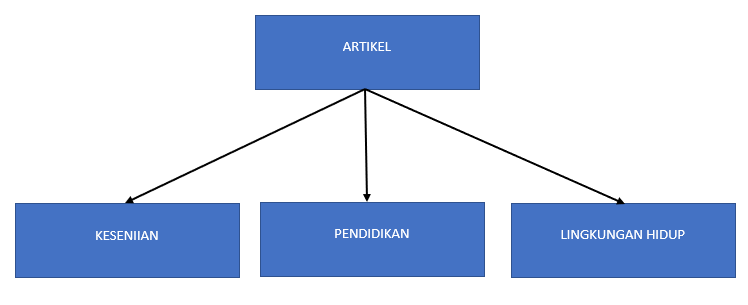
\includegraphics[scale=0.5]{figures/AIP/b1.PNG}
		\caption{Aip-Klasifikasi teks}
		\label{contoh}
	\end{figure}
	
\item Klasifikasi Bunga tidak dapat penggunakan machine learning
	\par Dikarenakan masalah dari input yang serupa namun output yang berbeda ‘noise’, yang dimaksud dengan noise adalah contoh pada output yang direkam bukan seperti perkiraan.
	\begin{figure}[ht]
		\centering
		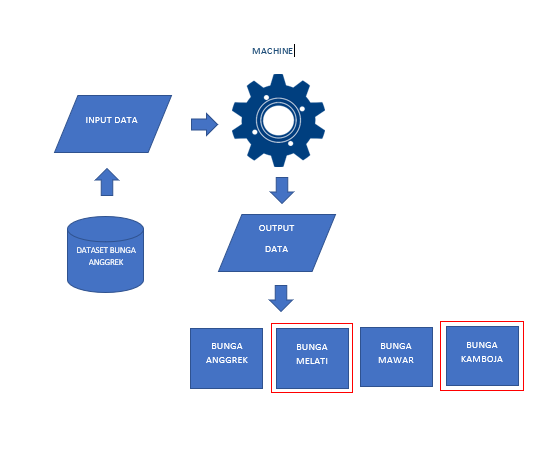
\includegraphics[scale=0.5]{figures/AIP/b2.PNG}
		\caption{Aip-Klasifikasi bunga}
		\label{contoh}
	\end{figure}

\item Teknik pembelajaran mesin pada teks YouTube
	\par Teknik Machine Learning pada YouTube memperhatikan apa saja yang menarik perhatian para penggunanya. Ketika kita sedang menonton di YouTube, pada sebelah kanan terdapat 'Up Next' yang menampilkan beberapa video serupa yang sedang ditonton. Dan ketika mengklik salah satu video dari baris tersebut, maka YouTube akan mengingatnya dan menggunakan kata yang tertera sebagai referensi.
	\begin{figure}[ht]
		\centering
		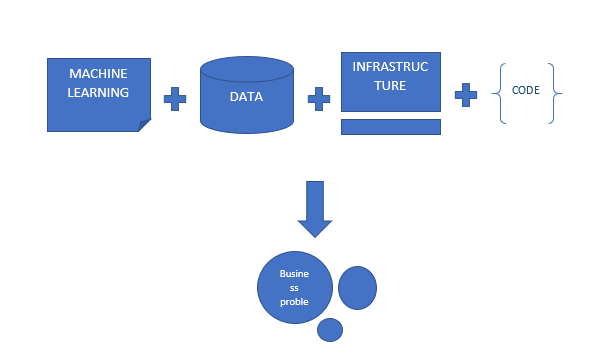
\includegraphics[scale=0.5]{figures/AIP/b3.PNG}
		\caption{Aip-Teknik YouTube}
		\label{contoh}
	\end{figure}

\item Vectorisasi Data
	\begin{itemize}
		\item Vectorisasi Data merupakan pemecahan serta pembagian data kemudian dilakukan perhitungan datanya.
	\end{itemize}
	
\item Bag of word
	\par Bag of Words adalah metode untuk mengekstraksi fitur dari dokumen teks.
	\begin{figure}[ht]
		\centering
		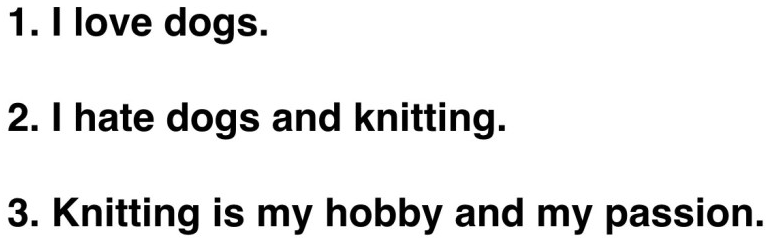
\includegraphics[scale=0.5]{figures/AIP/b4.PNG}
		\caption{Aip-Bag of Word}
		\label{contoh}
	\end{figure}
	
\item TF-IDF
	\par TF-IDF merupakan istilah beberapa frekuensi dokumen terbalik, adalah ukuran penilaian yang banyak digunakan dalam pengambilan informasi (IR) atau peringkasan. 
	\begin{figure}[ht]
		\centering
		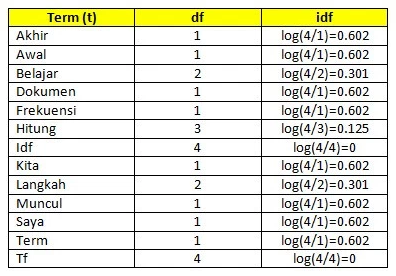
\includegraphics[scale=0.5]{figures/AIP/b5.PNG}
		\caption{Aip-TF IDF}
		\label{contoh}
	\end{figure}
\end{enumerate}




\section{Andi Muhammad Aslam/1164064}

\subsection{Teori}
\begin{enumerate}
\item Klasifikasi teks
	\par Klasifikasi merupakan kata serapan dari bahasa Belanda, classificatie, yang sendirinya berasal dari bahasa Prancis classification. Istilah ini menunjuk kepada sebuah metode untuk menyusun data secara sistematis atau menurut beberapa aturan atau kaidah yang telah ditetapkan.
	Di dalam KBBI, klasifikasi adalah penyusunan bersistem dalam kelompok atau golongan menurut kaidah atau standar yang ditetapkan. Secara harafiah bisa pula dikatakan bahwa klasifikasi adalah pembagian sesuatu menurut kelas-kelas. Menurut Ilmu Pengetahuan, Klasifikasi adalah Proses pengelompokkan benda berdasarkan ciri-ciri persamaan dan perbedaan.
	\begin{figure}[ht]
		\centering
		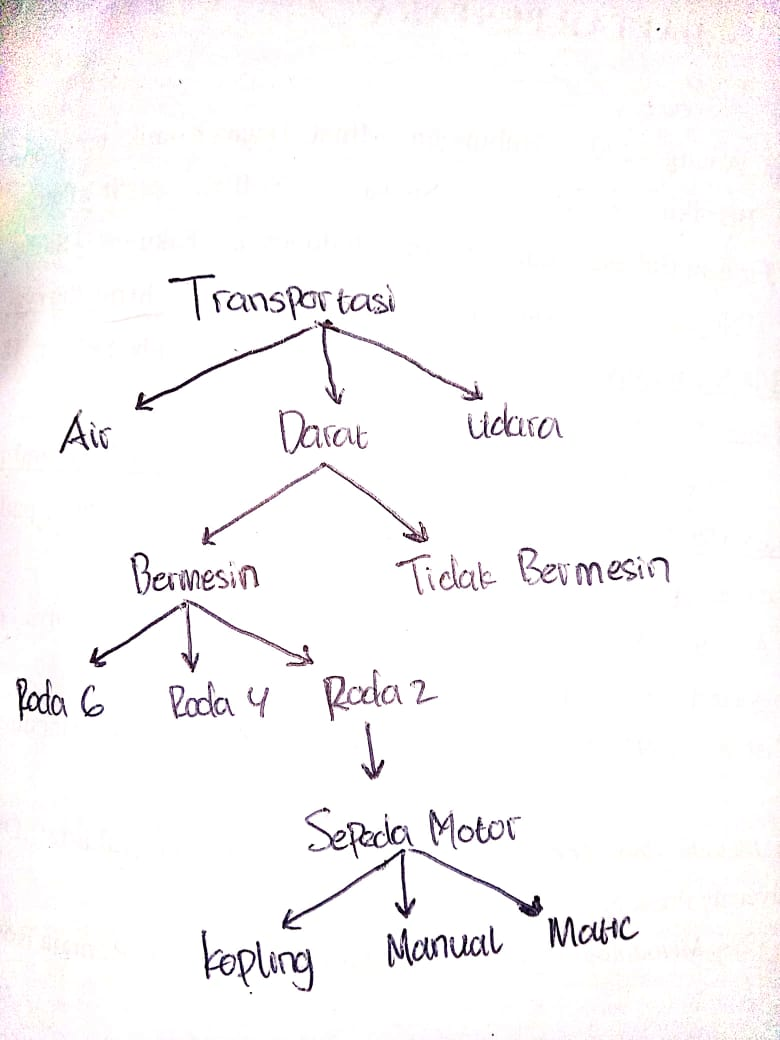
\includegraphics[scale=0.5]{figures/andi/4-1.jpeg}
		\caption{Klasifikasi teks}
		\label{Contoh Ilustrasi}
	\end{figure}
	
\item Klasifikasi Bunga tidak bisa menggunakan machine learning
	\par Machine Learning tidak dapat mengklasifikasikan bunga, Karena data yang diberikan pada 
mesin itu akan di algoritmakan untuk mencari sesuatu yang menarik dalam data yang kita 
berikan, hingga akhirnya sistem AI akan membangun pengetahuan berdasarkan data tersebut.
Dengan kata lain, pembelajaran mesin data beradaptasi terhadap suatu masalah dengan mempelajari pola-pola yang ditemukan dalam data
Sebagai contoh data pada spesies bunga dari genus Iris dengan melihat ukuran sepal (kelopak) dan petalnya(mahkota) pada algoritma data bunga tersebut akan melatih proses pembelajaran pada mesin dalam menganalisa spesies bunga Iris. Dan algoritma pembelajaran mesin akan mempelajari karakteristik dari masing-masing spesies bunga Iris berdasarkan ukuran sepal dan petal yang diberikan.
	\begin{figure}[ht]
		\centering
		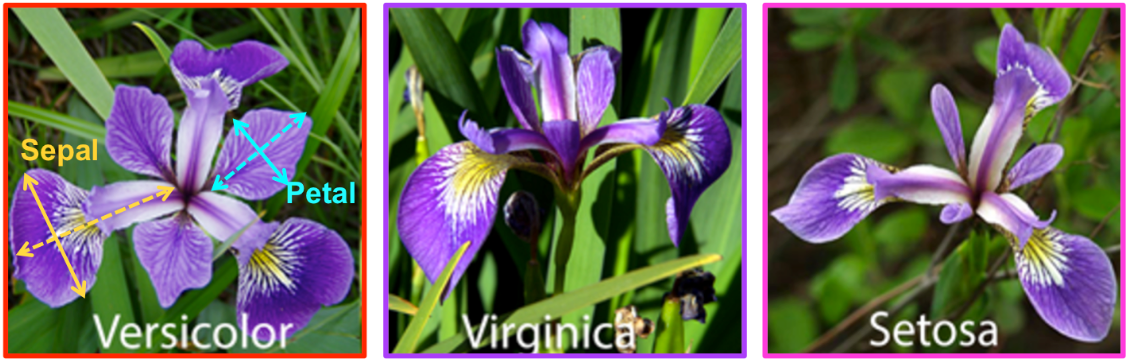
\includegraphics[scale=0.5]{figures/andi/4-2.png}
		\caption{Klasifikasi bunga}
		\label{Contoh Ilustrasi}
	\end{figure}

\item Youtube memungkinkan agar mendapatkan video yang direkomendasikan, karena Machine Learning pada Youtube pasti akan melibatkan data yang sering di lihat oleh penggunanya.
Youtube juga akan memberitahukan si pengguna apabila ada video baru yang telah di upload pada chanel yang direkomendasikan untuk si pengguna. Dan apabila menonton video pada youtube maka youtube dapat mengingat dan menggunakan kata tersebut sebagai referensi.
	\begin{figure}[ht]
		\centering
		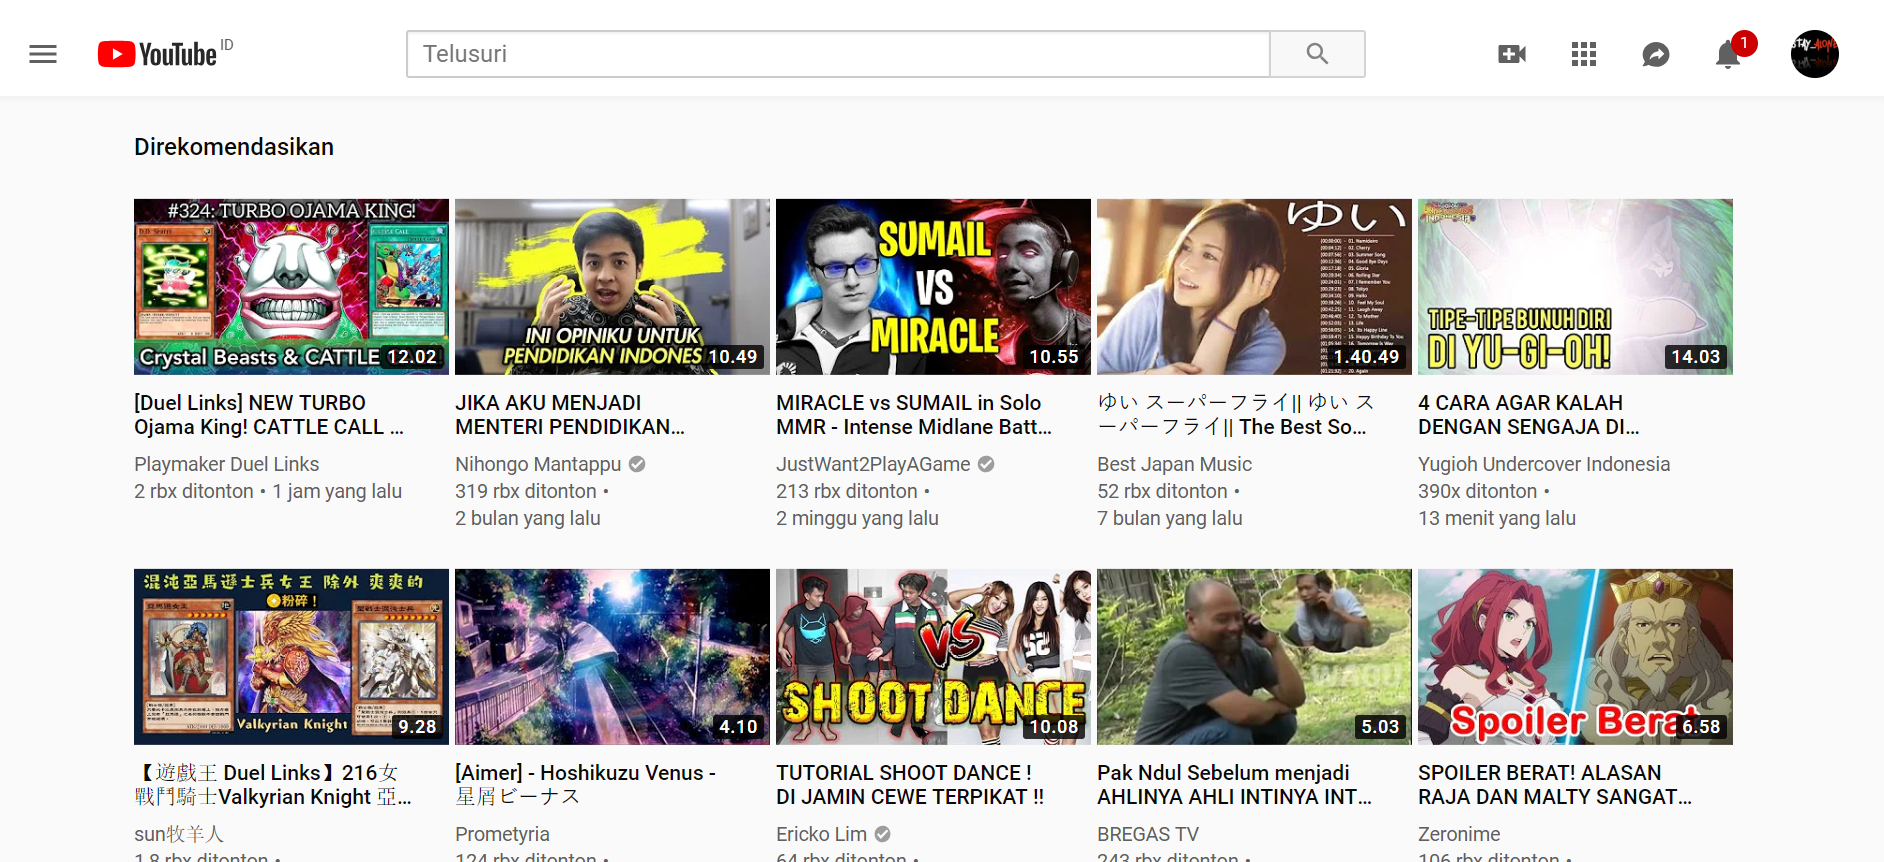
\includegraphics[scale=0.5]{figures/andi/4-3.PNG}
		\caption{Teknik YouTube}
		\label{Contoh Ilustrasi}
	\end{figure}

\item Vectorisasi Data
	\begin{itemize}
		\item proses vektorisasi ini menghasilkan suatu wujud peta yang menggambarkan keadaan permukaan bumi atau bentang alam. Sifat data yang geometris menunjukkan ukuran dimensi yang sesungguhnya.
	\end{itemize}
	
\item Bag of word
	\par Bag of word merupakan konsep yang diambil dari analisis, kemudian merepresentasikan dokumen berupa kumpulan informasi penting tanpa mengurutkan setiap katanya.
	\begin{figure}[ht]
		\centering
		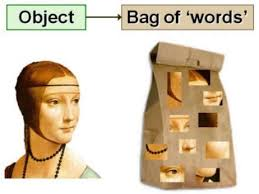
\includegraphics[scale=0.5]{figures/andi/4-5.jpg}
		\caption{Bag of Word}
		\label{Contoh Ilustrasi}
	\end{figure}
	
\item TF-IDF
	\par TF-IDF dimaksudkan untuk mencerminkan seberapa relevan suatu istilah dalam dokumen yang diberikan. Intuisi di baliknya adalah bahwa jika sebuah kata muncul beberapa kali dalam sebuah dokumen, kita harus meningkatkan relevansinya karena itu harus lebih bermakna daripada kata-kata lain yang muncul lebih sedikit kali (TF). Pada saat yang sama, jika sebuah kata muncul berkali-kali dalam suatu dokumen tetapi juga di sepanjang banyak dokumen lain, mungkin itu karena kata ini hanya kata yang sering; bukan karena itu relevan atau bermakna (IDF).
	\begin{figure}[ht]
		\centering
		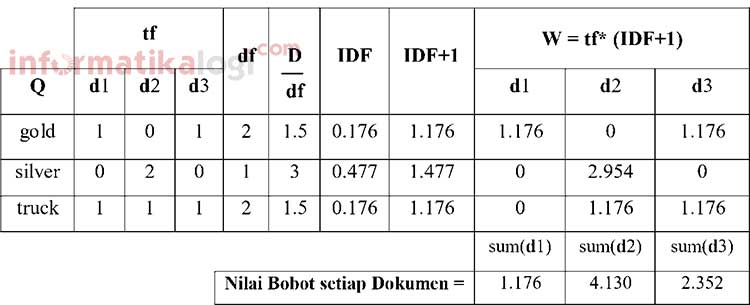
\includegraphics[scale=0.5]{figures/andi/4-6.jpg}
		\caption{TF-IDF}
		\label{Contoh Ilustrasi}
	\end{figure}
\end{enumerate}